\documentclass[letterpaper]{article}

\usepackage{style}  % If you feel like procrastinating, mess with this file
\usepackage{algo}   % Thank you Jeff, very cool!

\addbibresource{refs.bib}

% Required reading
% https://jmlr.csail.mit.edu/reviewing-papers/knuth_mathematical_writing.pdf
%   Along with required viewing:
%   https://www.youtube.com/watch?v=N6QEgbPWUrg&list=PLOdeqCXq1tXihn5KmyB2YTOqgxaUkcNYG
% https://faculty.math.illinois.edu/~west/grammar.html

% % % % % % % % % %
%     Cursor      %
%     Parking     %
%     Lot         %
% % % % % % % % % %

\title{Crypto}
\author{Anakin Dey}

\begin{document}
\maketitle

\section*{What is Cryptography?}

\begin{minipage}[c]{0.45\textwidth}
\begin{figure}[H]
  \centering
  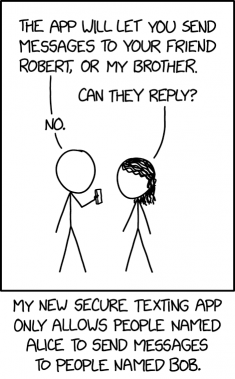
\includegraphics[width=0.5\textwidth]{alice_bob.png}
  \caption{From \cite{site:xkcd}}\label{fig:xkcd}
\end{figure}
\end{minipage}
\begin{minipage}[c]{0.5\textwidth}
Suppose that \emph{Alice} and \emph{Bob}, our two favorite protagonists, want to send messages to each other.
However, an eavesdropper, aptly named \emph{Eve}, wants to listen in and read these messages.
Alice and Bob want these messages to stay secret, for whatever reason (use your imagination).
The field of \emph{Cryptography} tells us all the ways Alice and Bob can (and can't) accomplish this.
\end{minipage}



\section*{Ye Olden Days}

Back in the before times, far before the first computers ever existed, \emph{Classical Ciphers} rules the land of codes and cryptography.
Classical ciphers rely on relatively simple techniques that can be executed by hand.
The \href{https://en.wikipedia.org/wiki/Caesar_cipher}{\emph{Caeser Cipher}} is arguable the most classical of the classical cipher.
It relies on a simple idea: shifting.
We take every letter and shift it by some fixed amount, wrapping around as necessary.
So if our shift amount was $4$ then we would have something like
\[
  A \mapsto E, B \mapsto F,  C \mapsto G, \ldots, U \mapsto Z, W \mapsto A, X \mapsto B, Y \mapsto C, Z \mapsto D
\]
So a simple message like ``sigpwny'' may get mapped to ``wmktarc.''

\subsection*{ASCII Values}

Messages are words made of letters.
Computers work with numbers.
The \href{https://www.asciitable.com/}{ASCII Table} tells us one of the most common ways to map a character to a unique number and also map any number to its corresponding character.
The Python programming language, the most commonly used language for cryptography, has some easy functions to quickly do this ASCII conversion.
The \mintinline{python}{ord} function takes in a character and returns its corresponding ASCII value.
So \mintinline{python}{ord("a")} returns $97$.
The function \mintinline{python}{chr} does the opposite by taking in a number and returning its corresponding character.
So \mintinline{python}{chr(97)} returns the character ``a.''

\subsection*{Modular Arithmetic Primer}
Since there are 26 letters ``a'' through ``z'' we can quickly computer the Caeser Cipher using what is call \emph{Modular Arithmetic} after representing our characters by numbers.
The letter ``a'' has an ASCII value of $97$ and the letter ``z'' has an ASCII value of $122$.
We can subtract $97$ from all the ASCII values and for now work with values between $0$ and $25$.
After we are done doing all of our shifts, we will just add $97$ back to each value and get the corresponding characters for those numbers.
For any values that are not lowercase letters, we will just ignore them.
So something like ``sigpwny\{\}'' gets mapped to ``wmktarc\{\}'' with a shift of $4$.

Modular arithmetic is arithmetic with remainders.
We fix some modulus $n$ throughout.
Since there are 26 letters, for our Caeser cipher we will use $n = 26$.
Every time we add and multiply two numbers $x$ and $y$, we will divide by $n$ and keep the remainder.
We will write this as $x + y \pmod{26}$.
So we have that $5 + 25 \equiv 30 \equiv 4 \pmod{26}$.
You may be familiar with this as the $\%$ operator in most programming languages.

Now with this prerequisite information, we can write a quick Python program to compute our Caeser cipher.
\begin{minted}{python}
message = "sigpwny"
shift = 4
ciphertext = ""
for c in message:           # loop through our message
    x = ord(c) - 97         # get ASCII and subtract 97
    x = (x + 4) % 26        # modular arithmetic!
    x += 97                 # Add 97
    ciphertext += chr(x)    # Convert back
print(ciphertext)           # Prints wmktarc
\end{minted}

However, you may already have an issue with seeing how insecure this is.
There are only $26$ possible shifts, $0$ through $25$.
So given some ciphertext that we know came from an English word, we can just bruteforce all possible shifts and just keep the one that looks like English.
For example, you know that the flags must contain the word ``sigpwny'' at the start!
This is why classical ciphers are no longer used.
Because computer are really, really fast at bruteforcing small combinations, classical ciphers are essentially useless.

\section*{One Time Pads}

One of the most basic modern cryptographic tools is the \emph{Exclusive-Or} operation, also called XOR.
In math it gets denoted by $x \oplus y$ and in Python we write \mintinline{python}{x ^ y}.
Say $x$ and $y$ are two bits, either $0$ or $1$.
The output of $x \oplus y$ is defined to be $1$ if and only if $x = 1$ or $y = 1$ but not both.
So we have the following table:
\begin{table}[H]
  \centering
  \begin{tabular}{c|c|c}
    $x$ & $y$ & $x \oplus y$ \\
    \hline
    $0$ & $0$ & $0$ \\
    $0$ & $1$ & $1$ \\
    $1$ & $0$ & $1$ \\
    $1$ & $1$ & $0$ \\
  \end{tabular}
  \caption{The truth table for $\oplus$}
  \label{tab:xor}
\end{table}

To apply this to whole messages $m$ with some key $k$, we convert the message to a bunch of bits in some method and just do this bit by bit.
So $0101 \oplus 1110 = 1010$.
There are a couple of properties that are easy to see.
For any $x, y, z$ we have that
\begin{enumerate}
\item $(x \oplus y) \oplus z = (x \oplus y) \oplus z$
\item $x \oplus y = y \oplus z$
\item $x \oplus x = 0$
\end{enumerate}
This means that $\oplus$ behaves like many operators in math we are used to and also has this very, very useful self cancellation property.

In the real world, there are a few considerations we have to take.
Messages may have different lengths.
The way this may be worked around is by making the shorter message the same length as the longer one by prepending $0$'s.
So $01 \oplus 11010 = 00001 \oplus 11010 = 11011$.
Another way to work around this is to repeat the shorter message until you reach the length of the longer message.
So $01 \oplus 11010 = 01010 \oplus 11010 = 10000$.
Note that these give different results.
These may be combined as well.
Sometimes you may have a key that you want to be 16 bytes long (8 bits to a single byte) but its only 15 bytes long.
You may pad the key with 8 0's to get up to 16 bytes and then repeat that key for every single 16 byte chunk of your message.

\section*{Bigger Numbers, Better Ciphers}

Modular arithmetic is much more useful than what was previously advertised when talking about classical ciphers.
A major theme of cryptography is the idea of a \emph{trapdoor}: something that is easy to enter one way but hard to escape from the other way.
Prime numbers give us this trapdoor.
It is incredibly easy for us (or rather, our computers) to multiply two numbers, even if those numbers are 512 bits long or even 1024 bits long.
However, factoring numbers into primes is computationally difficult.
This trapdoor will be the basis of the RSA cryptosystem, named after Rivest, Shamir, and Adleman.

\subsection*{Hidden Numbers}

One of the seemingly magical things about RSA is that it is an \emph{asymmetric} cryptosystem.
The sender of a message does not have to know the secret key to be able to successfully encrypt a message.
This seems paradoxical, but the math indeed does work out.
The goal of challenges like this will be to try to identify some, or all, of the secret information to be able decrypt the flag.

First two large primes $p$ and $q$ are chosen and kept secret.
Then, a value $n = p * q$ is computed and made public.
Remember, factoring is quite hard if $p$ and $q$ are large prime numbers.
Another secret value $\phi = (p - 1)(q - 1)$ is computed.
We have another public value $e$.
For a variety of reasons, none of which are important for now, usually $e = 2^{16} + 1 = 65537$.
Using $e$ and $\phi$, we compute $d$ which is the unique value such that $e * d \equiv 1 \pmod{\phi}$.
If you know $\phi$, this can be very easily computed using the Python \mintinline{python}{pow} function: \mintinline{python}{d = pow{e, -1, (p - 1)(q - 1)}}.
If you do not know $\phi$, then $d$ is essentially impossible to compute since you need to know $p$ and $q$.

In short, the secrets are primes $p, q$ and a value $\phi = (p - 1) (q - 1)$ and $d$ such that $ed \equiv 1 \pmod{\phi}$.
The numbers $n$ and $e$ are released to the public.

The \href{https://www.pycryptodome.org/}{PyCryptodome} library has some fantastic functions to convert bytes to a number and back: \mintinline{python}{bytes_to_long} and \mintinline{python}{long_to_bytes}.
So suppose our message $m$ is already in the form of some number.
Then the ciphertext number $c$ can be computed using the public information:
\[
  c \equiv m^{e} \pmod{n}.
\]
In Python, we can just compute \mintinline{python}{pow(m, e, n)}.
Decryption is just as simple:
\[
  m \equiv c^{d} \pmod{n}.
\]
Since $d$ is kept secret, only the intended recipient can decrypt the message assuming all the values such as $p$ and $q$ are chosen safely.

But if the values were chosen safely this wouldn't be a CTF, would it?

\section*{Big List of General Advice}

\begin{itemize}
\item Every challenge author has their own way of converting between messages and numbers and bytes and other data formats.
      Read the source code and make sure you know how these are being done and what objects you are working with.
      Whatever they are doing to convert the flag into workable data, doing the reverse of that should be part of your decryption.
\item Get out scratch paper.
      Actual scratch paper and maybe also a Python interpreter to quick test ideas.
      Math is not a spectator sport, get your hands dirty.
\item Google, Google, Google.
      This is self-explanatory.
\end{itemize}

\printbibliography
\end{document}
